\documentclass[aspectratio=169]{beamer}
\usepackage{amsmath,amssymb,bm}
\usepackage{graphicx}
\usepackage{tikz}
\usetikzlibrary{arrows.meta,positioning,shapes.geometric,fit}

\title{Deep Reinforcement Learning: Foundations to Systems}
\author{Academic Talk Draft}
\date{}

\begin{document}

% =========================
% STEP 3 — Part I slides
% =========================

\begin{frame}{Reinforcement Learning Problem Setting}
\begin{itemize}
  \item Agent observes $s_t$, chooses $a_t\sim\pi(a\mid s_t)$
  \item Environment returns $r_t$, transitions to $s_{t+1}\sim P(\cdot\mid s_t,a_t)$
  \item Trajectory: $\tau=(s_0,a_0,r_0,\dots)$
  \item Return: $G_t=\sum_{k=0}^{\infty}\gamma^k r_{t+k}$
  \item Objective: $J(\pi)=\mathbb{E}_{\tau\sim\pi}[G_0]$
\end{itemize}
% Note: Emphasize partial observability as extension to POMDP; keep MDP for notation.
\end{frame}

\begin{frame}{Markov Decision Processes (MDPs)}
\begin{itemize}
  \item MDP: $(\mathcal S,\mathcal A,P,R,\gamma)$
  \item Markov property: $P(s_{t+1}\mid s_{0:t},a_{0:t})=P(s_{t+1}\mid s_t,a_t)$
  \item Policy $\pi(a\mid s)$ induces a controlled Markov chain
  \item Reward model: $R(s,a)=\mathbb{E}[r_t\mid s_t=s,a_t=a]$
  \item Goal: find $\pi^*\in\arg\max_\pi J(\pi)$
\end{itemize}
% Note: Connect to stochastic control: discrete-time, discounted infinite horizon setting.
\end{frame}

\begin{frame}{Reinforcement Learning as Stochastic Control}
\begin{itemize}
  \item MDP $\Leftrightarrow$ discrete-time stochastic control system
  \item Value function $V^\pi$ $\Leftrightarrow$ cost-to-go under feedback law $\pi$
  \item Bellman equation $\Leftrightarrow$ dynamic programming principle
  \item Optimal policy $\pi^*(s)$ $\Leftrightarrow$ optimal feedback control
\end{itemize}
\[
V^*(s)=\sup_a\,\mathbb{E}\!\left[r(s,a)+\gamma V^*(s')\mid s,a\right]
\]
% Note: Frame RL as approximate dynamic programming on controlled Markov chains.
\end{frame}

\begin{frame}{Continuous-Time View}
\[
dX_t=b(X_t,a_t)\,dt+\sigma(X_t)\,dW_t
\]
\[
\sup_a\,\mathbb{E}\!\left[\int_0^\infty e^{-\rho t}r(X_t,a_t)\,dt\right]
\]
\[
\rho V(x)=\sup_a\left\{r(x,a)+\mathcal L^aV(x)\right\}
\]
\begin{itemize}
  \item Many RL methods are sampling-based approximations to DP/HJB solutions
\end{itemize}
% Note: Connect policy/value iteration to numerical PDE and stochastic approximation viewpoints.
\end{frame}

\begin{frame}{Bellman Expectation and Optimality Equations}
\begin{itemize}
  \item $V^\pi(s)=\mathbb{E}_\pi\!\left[\sum_{t\ge 0}\gamma^t r_t\mid s_0=s\right]$
  \item $Q^\pi(s,a)=\mathbb{E}_\pi\!\left[\sum_{t\ge 0}\gamma^t r_t\mid s_0=s,a_0=a\right]$
  \item Bellman expectation: $V^\pi(s)=\mathbb{E}[r+\gamma V^\pi(s')\mid s,\pi]$
  \item Bellman optimality: $V^*(s)=\max_a\mathbb{E}[r+\gamma V^*(s')\mid s,a]$
  \item $Q^*(s,a)=\mathbb{E}[r+\gamma\max_{a'}Q^*(s',a')\mid s,a]$
\end{itemize}
% Note: Mention contraction mapping under sup norm when gamma<1.
\end{frame}

\begin{frame}{Dynamic Programming Interpretation}
\begin{itemize}
  \item Policy evaluation: solve $V^\pi=T^\pi V^\pi$
  \item Policy improvement: $\pi'(s)\in\arg\max_a Q^\pi(s,a)$
  \item Policy iteration alternates evaluation and improvement
  \item Value iteration: $V_{k+1}=TV_k$
  \item Approximate DP replaces exact expectations by samples
\end{itemize}
% Note: Stress approximation error + sampling error decomposition.
\end{frame}

\begin{frame}{Q-Learning}
\begin{itemize}
  \item Off-policy TD control with bootstrapping
  \item Update:
  \[
  Q(s,a)\leftarrow Q(s,a)+\alpha\big[r+\gamma\max_{a'}Q(s',a')-Q(s,a)\big]
  \]
  \item Converges tabularly under GLIE and Robbins--Monro steps
  \item Uses replayed transitions in deep variants (DQN)
  \item Strength: simple, model-free, greedy improvement
\end{itemize}
% Note: Clarify maximization bias and Double Q-learning fix.
\end{frame}

\begin{frame}{Policy Gradient Theorem}
\begin{itemize}
  \item Parameterize policy: $\pi_\theta(a\mid s)$
  \item Performance objective: $J(\theta)=\mathbb{E}_{\tau\sim\pi_\theta}[G_0]$
  \item Theorem:
  \[
  \nabla_\theta J(\theta)=\mathbb{E}\big[\nabla_\theta\log\pi_\theta(a\mid s)\,Q^{\pi}(s,a)\big]
  \]
  \item Baseline $b(s)$ keeps unbiasedness, reduces variance
  \item REINFORCE uses Monte Carlo return estimators
\end{itemize}
% Note: Highlight score-function estimator and variance challenge.
\end{frame}

\begin{frame}{Actor--Critic Methods}
\begin{itemize}
  \item Actor updates policy; critic estimates $V^\pi$ or $Q^\pi$
  \item TD error: $\delta_t=r_t+\gamma V_\phi(s_{t+1})-V_\phi(s_t)$
  \item Actor step: $\theta\leftarrow\theta+\alpha_\theta\nabla_\theta\log\pi_\theta(a_t\mid s_t)\,\hat A_t$
  \item Critic step: minimize $\delta_t^2$ (or multi-step targets)
  \item Practical core: A2C/A3C, PPO, IMPALA
\end{itemize}
% Note: Emphasize bias-variance trade-off via bootstrapped advantage estimates.
\end{frame}

\begin{frame}{Deep Neural Function Approximation}
\begin{itemize}
  \item Replace tables by networks: $V_\phi(s), Q_\phi(s,a), \pi_\theta(a\mid s)$
  \item Enables high-dimensional observations (pixels, text, game states)
  \item Stabilization: target networks, replay buffers, normalization
  \item Representation learning couples control and feature extraction
  \item Risk: deadly triad (off-policy + bootstrap + approximation)
\end{itemize}
% Note: Bridge to Part II: engineering mitigations made this reliable at scale.
\end{frame}

% =========================
% STEP 4 — Part II slides
% =========================

\begin{frame}{AlphaGo --- Algorithmic Core}
\begin{itemize}
  \item Setting: Go; perfect information, huge branching factor
  \item RL core: policy gradient fine-tuning + value learning
  \item Networks: policy CNN + value CNN on board tensors
  \item Search: MCTS combines policy priors + rollout/value evaluation
  \item Self-play used for policy/value refinement
\end{itemize}
% Note: Scaling axis here is search coupled with learned evaluation.
\end{frame}

\begin{frame}{AlphaGo --- Engineering and Scale}
\begin{itemize}
  \item Data: $\sim 30$M expert positions + large self-play corpus
  \item Compute: distributed CPU rollouts + multi-GPU training
  \item Match-time scale: thousands of MCTS simulations per move
  \item Tricks: fast rollout policy, asynchronous self-play/training
  \item Key lesson: search quality $\times$ learned priors beats raw policy inference
\end{itemize}
% Note: Emphasize effective branching-factor reduction by policy/value guidance.
\end{frame}

\begin{frame}{AlphaGo Zero --- Algorithmic Core}
\begin{itemize}
  \item Setting: Go from scratch; no expert demonstrations
  \item RL core: generalized policy iteration via self-play + MCTS
  \item Network: single residual net outputs $(p_\theta,v_\theta)$
  \item MCTS visit counts define improved policy targets
  \item Closed loop: self-play $\rightarrow$ update $\rightarrow$ stronger self-play
\end{itemize}
% Note: Highlight pure self-play policy iteration viewpoint.
\end{frame}

\begin{frame}{AlphaGo Zero --- Engineering and Scale}
\begin{itemize}
  \item Data: all training data generated online by self-play
  \item Compute: TPU-based training + large parallel game generation
  \item Timeline: superhuman level reached within days of training
  \item Tricks: replay windowing, regularized loss, gating by match tests
  \item Key lesson: self-play can be a fully autonomous data engine
\end{itemize}
% Note: Scaling axis is data freshness and iterative improvement, not labels.
\end{frame}

\begin{frame}{OpenAI Five --- Algorithmic Core}
\begin{itemize}
  \item Setting: Dota 2; partial observability, long horizon, 5v5 coordination
  \item RL core: PPO with recurrent actor-critic policies
  \item Architecture: LSTM policy/value with action masking
  \item Training regime: self-play in an evolving opponent league
  \item Objective shaping supports sparse delayed win signal
\end{itemize}
% Note: Connect to stochastic control with partial observation and constraints.
\end{frame}

\begin{frame}{OpenAI Five --- Engineering and Scale}
\begin{itemize}
  \item Throughput: up to $\sim 180$ years of simulation per day
  \item Resources: very large distributed CPU+GPU cluster
  \item Duration: months of continual training and league updates
  \item Tricks: PPO stabilization, curriculum, reward shaping, policy lag control
  \item Key lesson: simulation throughput is the dominant control knob
\end{itemize}
% Note: Scaling axis is distributed on-policy data generation at extreme rate.
\end{frame}

\begin{frame}{Quake III Arena MARL --- Algorithmic Core}
\begin{itemize}
  \item Setting: capture-the-flag; mixed cooperation and competition
  \item RL core: off-policy multi-agent RL with population-based training
  \item Architecture: recurrent agents with shared backbone + role conditioning
  \item Training uses teammate/opponent sampling across a population
  \item Population diversity mitigates non-stationarity
\end{itemize}
% Note: Emphasize league/population design as algorithmic component.
\end{frame}

\begin{frame}{Quake III Arena MARL --- Engineering and Scale}
\begin{itemize}
  \item Scale: large distributed actor pool generating diverse trajectories
  \item Opponents: continually refreshed league for robust policy improvement
  \item Environment randomization broadens tactical coverage
  \item Tricks: PBT hyperparameter mutation + matchmaking schedules
  \item Key lesson: diversity of training interactions drives robustness
\end{itemize}
% Note: Scaling axis is population diversity, not only per-policy compute.
\end{frame}

\begin{frame}{RL for Formal Reasoning (AlphaProof) --- Algorithmic Core}
\begin{itemize}
  \item Setting: formal theorem proving as sequential decision process
  \item RL core: policy/value-guided tree search over proof states
  \item Architecture: neural proposer for tactics + value/priority estimator
  \item Environment: proof assistant verifier gives exact validity feedback
  \item Test-time search adapts computation per theorem difficulty
\end{itemize}
% Note: Frame as planner+learner loop with symbolic constraints.
\end{frame}

\begin{frame}{RL for Formal Reasoning (AlphaProof) --- Engineering and Scale}
\begin{itemize}
  \item Data: millions of synthetic/curated proof trajectories
  \item Compute: large-scale distributed search + accelerator training
  \item Runtime scale: many candidate proof branches explored per problem
  \item Tricks: verifier-grounded rewards, curriculum, offline-to-online fine-tuning
  \item Key lesson: search with verifier feedback enables reliable RL signals
\end{itemize}
% Note: Scaling axis is verifier-grounded search with adaptive test-time compute.
\end{frame}

\begin{frame}{Deep RL Milestones}
\centering
\begin{tabular}{ll}
\textbf{2013} & DQN \\
\textbf{2016} & AlphaGo \\
\textbf{2017} & AlphaGo Zero \\
\textbf{2019} & OpenAI Five \\
\textbf{2019} & Quake III Arena MARL \\
\textbf{2025} & RL for formal mathematical reasoning
\end{tabular}
\begin{itemize}
  \item Trend: increasing scale, self-play, search, and systems engineering
\end{itemize}
% Note: Use as chronology anchor before systems/engineering synthesis.
\end{frame}

\begin{frame}{Why Did Deep RL Accelerate After 2015?}
\begin{itemize}
  \item GPUs/TPUs enabled large-batch optimization and rapid iteration
  \item Rich simulators supplied cheap, resettable, parallel experience
  \item Deep networks learned reusable representations from raw observations
  \item Self-play created endogenous curricula in competitive domains
  \item Distributed training synchronized actors, learners, and evaluation leagues
\end{itemize}
% Note: This is the unifying mechanism behind post-2015 milestone systems.
\end{frame}

% =========================
% STEP 5 — Diagram slides (TikZ)
% =========================

\begin{frame}{Diagram: RL Agent--Environment Loop}
\centering
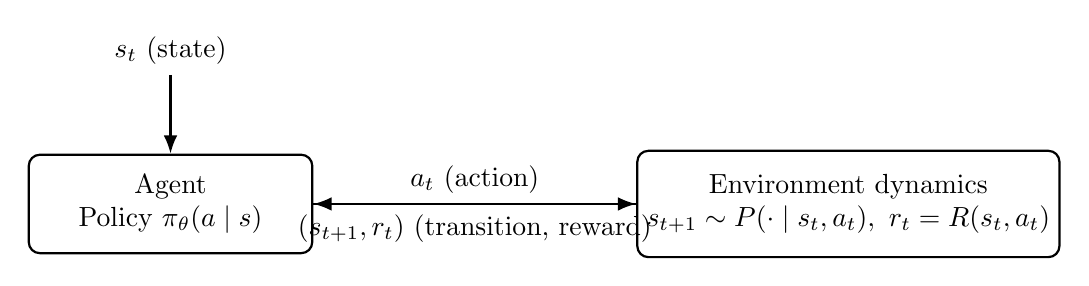
\begin{tikzpicture}[>=Latex,thick,node distance=2.8cm]
  \node[draw,rounded corners,minimum width=3.6cm,minimum height=1.25cm,align=center] (agent) {Agent\\Policy $\pi_\theta(a\mid s)$};
  \node[draw,rounded corners,right=4.1cm of agent,minimum width=4.4cm,minimum height=1.35cm,align=center] (env) {Environment dynamics\\$s_{t+1}\sim P(\cdot\mid s_t,a_t),\ r_t=R(s_t,a_t)$};

  \draw[->] (agent) -- node[above] {$a_t$ (action)} (env);
  \draw[->] (env) -- node[below] {$(s_{t+1},r_t)$ (transition, reward)} (agent);

  \node[above=1.0cm of agent,align=center] (state) {$s_t$ (state)};
  \draw[->] (state) -- (agent);
\end{tikzpicture}
% Note: Explicitly separates control law, dynamics, transition kernel, and reward channel.
\end{frame}

\begin{frame}{Diagram: AlphaGo Training Pipeline}
\centering
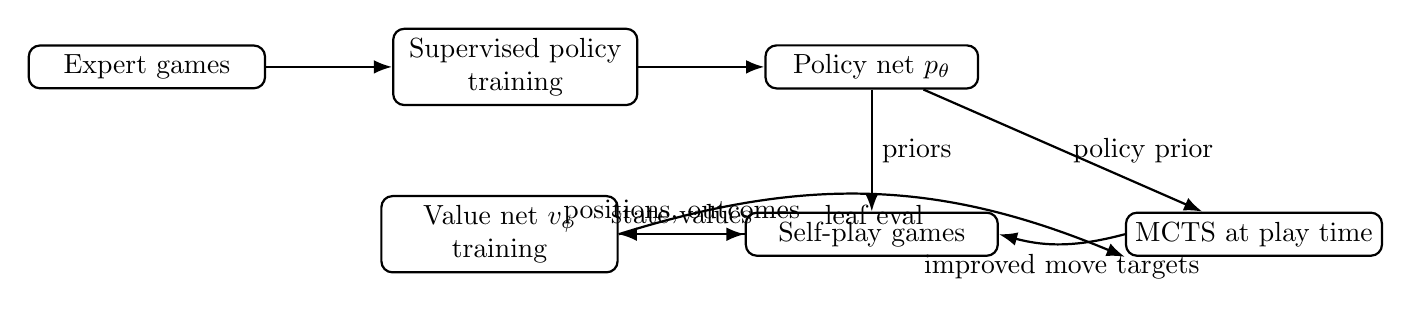
\begin{tikzpicture}[>=Latex,thick,node distance=1.55cm and 1.6cm]
  \node[draw,rounded corners,minimum width=3.0cm,align=center] (expert) {Expert games};
  \node[draw,rounded corners,right=of expert,minimum width=3.1cm,align=center] (sup) {Supervised policy\\training};
  \node[draw,rounded corners,right=of sup,minimum width=2.7cm,align=center] (pol) {Policy net $p_\theta$};

  \node[draw,rounded corners,below=of pol,minimum width=3.2cm,align=center] (selfplay) {Self-play games};
  \node[draw,rounded corners,left=of selfplay,minimum width=3.0cm,align=center] (value) {Value net $v_\phi$\\training};
  \node[draw,rounded corners,right=of selfplay,minimum width=3.0cm,align=center] (mcts) {MCTS at play time};

  \draw[->] (expert) -- (sup);
  \draw[->] (sup) -- (pol);
  \draw[->] (pol) -- node[right] {priors} (selfplay);
  \draw[->] (selfplay) -- node[above] {positions, outcomes} (value);
  \draw[->] (value) -- node[above] {state values} (selfplay);

  \draw[->] (pol) -- node[right] {policy prior} (mcts);
  \draw[->] (value.east) to[bend left=20] node[below] {leaf eval} (mcts.south west);
  \draw[->] (mcts.west) to[bend left=15] node[below] {improved move targets} (selfplay.east);
\end{tikzpicture}
% Note: Makes supervised bootstrap, self-play improvement, value learning, and inference-time MCTS explicit.
\end{frame}

\begin{frame}{Diagram: Large-Scale Distributed RL Pipeline}
\centering
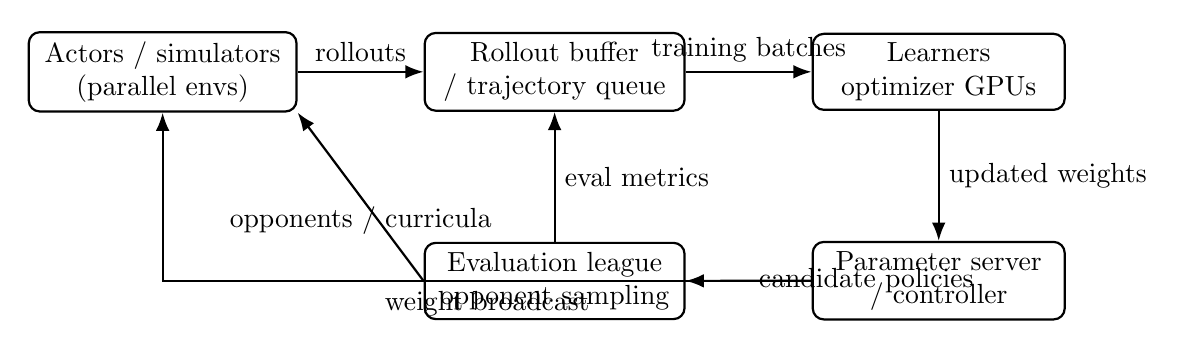
\begin{tikzpicture}[>=Latex,thick,node distance=1.65cm and 1.6cm]
  \node[draw,rounded corners,minimum width=3.4cm,align=center] (actors) {Actors / simulators\\(parallel envs)};
  \node[draw,rounded corners,right=of actors,minimum width=3.3cm,align=center] (queue) {Rollout buffer\\/ trajectory queue};
  \node[draw,rounded corners,right=of queue,minimum width=3.2cm,align=center] (learners) {Learners\\optimizer GPUs};
  \node[draw,rounded corners,below=of learners,minimum width=3.2cm,align=center] (ctrl) {Parameter server\\/ controller};
  \node[draw,rounded corners,below=of queue,minimum width=3.3cm,align=center] (league) {Evaluation league\\opponent sampling};

  \draw[->] (actors) -- node[above] {rollouts} (queue);
  \draw[->] (queue) -- node[above] {training batches} (learners);
  \draw[->] (learners) -- node[right] {updated weights} (ctrl);
  \draw[->] (ctrl.west) -| node[pos=0.25,below] {weight broadcast} (actors.south);

  \draw[->] (ctrl) -- node[right] {candidate policies} (league);
  \draw[->] (league.west) -- node[below] {opponents / curricula} (actors.south east);
  \draw[->] (league.north) -- node[right] {eval metrics} (queue.south);
\end{tikzpicture}
% Note: Shows end-to-end dataflow, policy distribution, and league-driven opponent selection.
\end{frame}


% =========================
% STEP 6 — Conclusion slides
% =========================

\begin{frame}{Engineering Lessons from Modern Reinforcement Learning}
\begin{itemize}
  \item Self-play provides an adaptive curriculum tied to policy strength
  \item Search + learning hybrids improve decisions under limited horizon
  \item Reward shaping and environment design determine signal quality
  \item Distributed simulation is often the primary scaling bottleneck
  \item Scaling data/compute is a systems co-design problem, not tuning
\end{itemize}
% Note: Emphasize reusable engineering principles behind major RL breakthroughs.
\end{frame}

\begin{frame}{Open Questions for Stochastic Control Researchers}
\begin{itemize}
  \item Continuous-time RL: consistent discretization limits and error bounds
  \item Exploration in high dimensions with structure-aware guarantees
  \item Sample efficiency via models, priors, and uncertainty quantification
  \item Stability/convergence under nonlinear function approximation
  \item Links to HJB, BSDE, mean-field control, and robust control
\end{itemize}
% Note: Conclude that RL is a computational continuation of stochastic control.
\end{frame}

\end{document}
